  \let\negmedspace\undefined
\let\negthickspace\undefined
\documentclass[journal]{IEEEtran}
\usepackage[a5paper, margin=10mm, onecolumn]{geometry}
\usepackage{lmodern} % Ensure lmodern is loaded for pdflatex
\usepackage{tfrupee} % Include tfrupee package

\setlength{\headheight}{1cm} % Set the height of the header box
\setlength{\headsep}{0mm}     % Set the distance between the header box and the top of the text

\usepackage{gvv-book}
\usepackage{gvv}
\usepackage{cite}
\usepackage{amsmath,amssymb,amsfonts,amsthm}
\usepackage{algorithmic}
\usepackage{graphicx}
\usepackage{textcomp}
\usepackage{xcolor}
\usepackage{txfonts}
\usepackage{listings}
\usepackage{enumitem}
\usepackage{mathtools}
\usepackage{gensymb}
\usepackage{comment}
\usepackage[breaklinks=true]{hyperref}
\usepackage{tkz-euclide} 
\usepackage{listings}                                      
\def\inputGnumericTable{}                                 
\usepackage[latin1]{inputenc}                                
\usepackage{color}                                            
\usepackage{array}                                            
\usepackage{longtable}
\usepackage{multicol}
\usepackage{calc}                                             
\usepackage{multirow}                                         
\usepackage{hhline}                                           
\usepackage{ifthen}                                           
\usepackage{lscape}
\begin{document}
	
	\bibliographystyle{IEEEtran}
	\vspace{3cm}
	
	\title{11.16.3.8.8}
	\author{EE24BTECH11063 - Y. Harsha Vardhan Reddy }
	% \maketitle
	% \newpage
	% \bigskip
	{\let\newpage\relax\maketitle}
	
	\renewcommand{\thefigure}{\theenumi}
	\renewcommand{\thetable}{\theenumi}
	\setlength{\intextsep}{10pt} % Space between text and floats
	
	
	\numberwithin{equation}{enumi}
	\numberwithin{figure}{enumi}
	\renewcommand{\thetable}{\theenumi}
	
	
\textbf{Question}:\\
Find the probability that no toss results in a tail when coin is tossed thrice(independent tosses) \\
\textbf{Solution: }\\
\textbf{Theoretical solution: }\\
To calculate the probability of getting all three tails when a coin is tossed three times:

\begin{itemize}
    \item The probability of getting a tail (\(T\)) in a single toss is:
    \[
    P(T) = \frac{1}{2}.
    \]
    \item Since the tosses are independent, the probability of getting three tails (\(TTT\)) is given by:
    \[
    P(\text{Three Tails}) = P(T) \times P(T) \times P(T).
    \]
    \item Substituting \(P(T) = \frac{1}{2}\), we have:
    \[
    P(\text{Three Tails}) = \left(\frac{1}{2}\right)^3 = \frac{1}{8}.
    \]
\end{itemize}

Thus, the probability of getting all three tails is:
\[
\boxed{\frac{1}{8}}
\]
\textbf{Computational solution: }\\


\section*{Z-Transform Computational Method for Coin Toss PMF}
\subsection*{PMF for a Single Coin Toss}
For a single coin toss, the probability mass function (PMF) is:
\[
P_X(k) =
\begin{cases}
p, & \text{if } x = 1 \text{ (Tails)} \\
1-p, & \text{if } x = 0 \text{ (Heads)}
\end{cases}
\]
where \(p = 0.5\) for a fair coin.

\subsection*{Conditions for PMF}
A valid PMF must satisfy the following conditions:
\begin{enumerate}
    \item Non-negativity: \(\forall k, P_X(k) \geq 0\).
    \item Normalization: \(\sum_{k} P_X(k) = 1\).
\end{enumerate}
For a single coin toss:
\begin{align}
P_X(0) + P_X(1) = 1.
\end{align}
Substituting \(p = 0.5\):
\begin{align}
P_X(0) = 0.5, \quad P_X(1) = 0.5.
\end{align}

\subsection*{Z-Transform Expansion}
The Z-transform for the number of tails in \(n\) coin tosses is given by:
\begin{align}
T(z) = \left( p + (1-p)z \right)^n
\end{align}
where:
\begin{itemize}
    \item \(p\) is the probability of tails (\(p = 0.5\) for a fair coin),
    \item \(1-p\) is the probability of heads (\(1-p = 0.5\) for a fair coin),
    \item \(n\) is the number of tosses (\(n = 3\)).
\end{itemize}
For $n=1$,
\begin{align}
T(z) = \left( p + (1-p)z \right)
\end{align}
For a fair die,
\begin{align}
P_X(0) = 0.5, \quad P_X(1) = 0.5,
\end{align}
\subsection*{Expansion of \(T(z)\)}
Expand the expression \(\left( p + (1-p)z \right)^n\) using the binomial theorem:
\begin{align}
T(z) = \sum_{k=0}^{n} \binom{n}{k} p^{n-k} (1-p)^k z^k
\end{align}
where:
\begin{itemize}
    \item \(\binom{n}{k}\) is the binomial coefficient, computed as:
    \begin{align}
    \binom{n}{k} = \frac{n!}{k! (n-k)!}
    \end{align}
    \item The coefficient of \(z^k\) in \(T(z)\) gives the probability \(P_X(k)\), where \(X\) is the number of tails.
\end{itemize}

\subsection*{Probability Mass Function (PMF)}
The PMF is computed as:
\begin{align}
P_X(k) = \binom{n}{k} p^{n-k} (1-p)^k
\end{align}
Substitute \(p = 0.5\) and \(1-p = 0.5\) for a fair coin:
\begin{align}
P_X(k) = \binom{n}{k} (0.5)^n
\end{align}

\subsection*{Computational Steps}
For each \(k \in \{0, 1, \dots, n\}\):
\begin{enumerate}
    \item Compute the binomial coefficient:
    \begin{align}
    \binom{n}{k} = \prod_{i=0}^{k-1} \frac{n-i}{k-i}
    \end{align}
    \item Multiply by \((0.5)^n\) to compute \(P_X(k)\):
    \begin{align}
    P_X(k) = \binom{n}{k} \cdot (0.5)^n
    \end{align}
\end{enumerate}

\subsection*{Result for \(n = 3\)}
Substituting \(n = 3\) and expanding:
\begin{align}
T(z) = (0.5 + 0.5z)^3 = 0.125 + 0.375z + 0.375z^2 + 0.125z^3
\end{align}
The PMF values are:
\begin{align}
P_X(0) = 0.125, \quad P_X(1) = 0.375, \quad P_X(2) = 0.375, \quad P_X(3) = 0.125
\end{align}
The CDF must satisfy:
\begin{enumerate}
    \item \(F_X(k)\) is non-decreasing.
    \item \(F_X(k) \in [0, 1]\) for all \(k\).
    \item \(F_X(n) = 1\), where \(n\) is the maximum number of tails.
\end{enumerate}
\subsection*{CDF Calculation}
The CDF is:
\begin{align}
F_X(k) = \sum_{i=0}^{k} P_X(i).
\end{align}

Compute the values:
\begin{align}
F_X(0) = P_X(0) = 0.125,
\end{align}
\begin{align}
F_X(1) = P_X(0) + P_X(1) = 0.125 + 0.375 = 0.5,
\end{align}
\begin{align}
F_X(2) = F_X(1) + P_X(2) = 0.5 + 0.375 = 0.875,
\end{align}
\begin{align}
F_X(3) = F_X(2) + P_X(3) = 0.875 + 0.125 = 1.
\end{align}
For \(n = 3\), the CDF values are:
\begin{align}
F_X(0) = 0.125, \quad F_X(1) = 0.5, \quad F_X(2) = 0.875, \quad F_X(3) = 1.
\end{align}


\subsection*{Probability of \(X = 3\)}
Using the CDF, the probability of \(X = 3\) is:
\begin{align}
P_X(3) = F_X(3) - F_X(2).
\end{align}

Substitute the values:
\begin{align}
P_X(3) = 1 - 0.875 = 0.125.
\end{align}
\subsection*{Conclusion}
The probability of getting all three tails is:
\[
P(X = 3) = \boxed{0.125}.
\]
	\begin{figure}[h!]
		\centering
		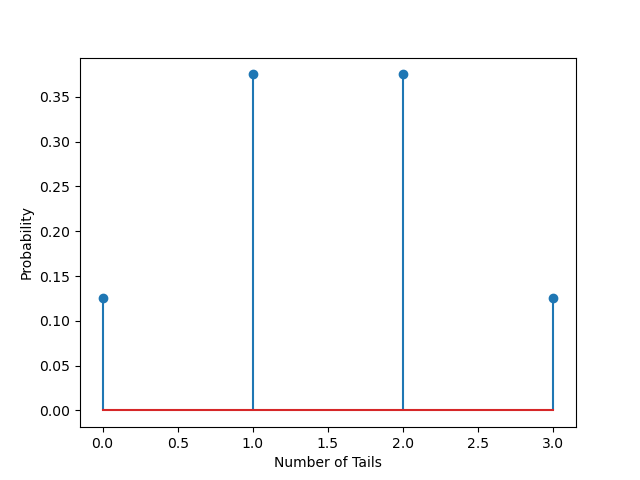
\includegraphics[width=\columnwidth]{figs/fig1.png}
		\label{stemplot}
	\end{figure}
	
\end{document}  
